% $Header: /cvsroot/latex-beamer/latex-beamer/solutions/conference-talks/conference-ornate-20min.en.tex,v 1.7 2007/01/28 20:48:23 tantau Exp $
\documentclass[14pt]{beamer}

\newcommand{\strong}[1]{{\normalfont\fontseries{b}\selectfont #1}}
\newcommand{\class}[1]{\mbox{\textsf{#1}}}
\newcommand{\func}[1]{\mbox{\texttt{#1()}}}
\newcommand{\code}[1]{\mbox{\texttt{#1}}}
\newcommand{\pkg}[1]{\strong{#1}}
\newcommand{\samp}[1]{`\mbox{\texttt{#1}}'}
\newcommand{\proglang}[1]{\textsf{#1}}
\newcommand{\putat}[3]{\begin{picture}(0,0)(0,0)\put(#1,#2){#3}\end{picture}}


\usepackage{beamerthemeAmsterdam}
\usepackage{relsize}
\usepackage{natbib}
\renewcommand{\bibsection}{\subsubsection*{\bibname } }
\def\newblock{}

\mode<presentation>
{
  \usetheme{Amsterdam}
}


\usepackage[english]{babel}

\usepackage[latin1]{inputenc}

\usepackage{times}
\usepackage[T1]{fontenc}
\usepackage[absolute,overlay]{textpos}
\newenvironment{reference}[2]{
  \begin{textblock*}{\textwidth}(#1,#2)
    \footnotesize\it\bgroup\color{black!50!black}}{\egroup\end{textblock*}}

\usepackage{graphics}
% Or whatever. Note that the encoding and the font should match. If T1
% does not look nice, try deleting the line with the fontenc.


%\title{Babelstream\smaller{\smaller{\smaller{{\texttrademark}}}}: 
\title{Statistical Consulting (BIS 578) Lecture 1}


\author{Michael J. Kane}

\date{}

\begin{document}

\begin{frame}
  \titlepage
\end{frame}

\begin{frame}{Outline for today's class}
  \tableofcontents
%  \let\thefootnote\relax\footnotetext{\relsize{-3}{The Research Plan and 
%    Plan of Study sections are adapted from slides provided by James Dziura  \\
%    }}
\end{frame}

\section{Collaborating with an investigator}

\subsection*{}

\begin{frame}{Why is it important for investigators to collaborate 
with us?}
``Clinical researchers rely on biostatisticians in order to design, conduct and 
analyse observational and experimental studies involving populations of 
subjects.'' \citep{Bangdiwala2001}
\end{frame}

\begin{frame}{We increase the rigor and provide new directions
for investigations}
``Early collaboration between the clinical investigator and statistician can 
improve the study design and validity of the results by developing the 
statistical methodology that specifically addresses the research hypothesis.''
\cite{Adams2009}
\end{frame}

\begin{frame}{OK, they need us...  Do we need them?}
Why is it important for us to collaborate with investigators?
\end{frame}

\begin{frame}{Of course we do.}
Investigator spend a lot of time acquiring domain knowledge and intuition

\vspace{0.5cm}

New data challenges provide inspiration for new theory
\end{frame}

\begin{frame}{Understanding your role}
Investigator
\begin{itemize}
\item Provides a general question for investigation
\item Provides domain knowledge
\end{itemize}
Statistician
\begin{itemize}
\item Shapes the investigators question into something that can be answered
  quantitatively
\item Provides a quantitative tools to answer the research question
\end{itemize}
\end{frame}

\begin{frame}{Goals of the Investigator and Statistican at the beginning of
a collaboration}
\begin{itemize}
\item Create a Research Question which tells what question the investigation 
  will answer
\item Create a Plan of Study which tells how the question will be answered
\end{itemize}
\end{frame}

\section{Coming up with a Research Question and Plan of Study}

\subsection{The Research Question}

\begin{frame}{The Research Question}
``The research question is the uncertainty about something in the population
that the investigator wants to resolve by making measurements on her
study subjects.'' \cite{Hulley2001}
\begin{figure}
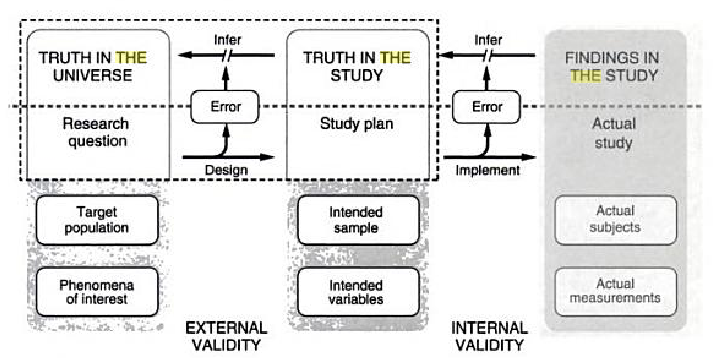
\includegraphics[width=3in]{Screenshot.png}
\end{figure}
\end{frame}

\begin{frame}{The importance of a clearly defined research question}
``Well-crafted questions guide the systematic planning of research.  
Formulating your questions precisely enables you to design a study with a 
good chance of answering them.'' \cite{Light1990}
\end{frame}

\begin{frame}{Creating a Research Question}
Creating a Research Question is an iterative process to shape and narrow
a question into an answerable format.
\end{frame}

\begin{frame}{Examples of Research Questions}
\begin{itemize}
\item Do phrophylactic antibiotics reduce the incidence of wound infection?
\item Does the use of ciprofloxacin reduce the incidence of infection 
  associated with puncture wounds to the foot in healthy, non-diabetic patients?
\end{itemize}
\end{frame}

\begin{frame}{Hulley \cite{Hulley2001} give 5 characteristics of a good
Research Question}
\begin{itemize}
\item Feasible
\item Interesting
\item Novel
\item Ethical
\item Relevant
\end{itemize}
\end{frame}

\begin{frame}{Feasible}
\begin{itemize}
\item Adequate number of subjects
\item Adequate technical expertise
\item Affordable in time in money
\item Manageable in scope
\end{itemize}
\end{frame}

\begin{frame}{Interesting}
\begin{itemize}
\item Getting the answers intrigues the investigator and her friends
\end{itemize}
\end{frame}

\begin{frame}{Novel}
\begin{itemize}
\item Confirms, refutes or extends previous findings
\item Provides new findings
\end{itemize}
\end{frame}

\begin{frame}{Ethical}
\begin{itemize}
\item Amenable to a study that instructional review board will approve
\end{itemize}
\end{frame}

\begin{frame}{Relevant}
\begin{itemize}
\item To scientific knowledge
\item To clinical and health policy
\item To future research
\end{itemize}
\end{frame}

\subsection{The Plan of Study}

\begin{frame}{The Plan of Study}
The Plan of Study tells how the Research Question will be answered.
\begin{itemize}
\item Clearly links to the Research Question
\item Identifies the target population
\item Identifies the outcome variables and key predictors of those variables
\item Identifies the type of study needed
\item Identifies background characteristics that might influence outcomes
\end{itemize}
\end{frame}

\begin{frame}{What do the Research Question and Plan of Study provide?}
\begin{itemize}
\item Promotes clarity of thought
\item Guides the production of a study protocol
\item Informs the choice of research methodology
\item Guides the analysis
\item Increases the likelihood of publication
\end{itemize}
\end{frame}

\section{Bibliography}

\subsection*{}

\begin{frame}[allowframebreaks]{Bibliography}
\bibliographystyle{alpha}
\bibliography{references.bib}
\end{frame}

\end{document}


